\chapter{Background and related work: Quality control and machine Learning} \label{Background and related work: Quality control and machine Learning}
\minitoc

\section{Introduction}

Product and process failures anticipation have been the subject of multiple researches for decades. Since the introduction of the Statistical Process Control (SPC) in the early 1920s by Walter A. Shewart multiple methods have been proposed to monitor and control a process. From univariate Shewhart and  CUSUM \citep{woodall1985multivariate} \citep{crosier1988multivariate} control charts to multivariate methods such as Hotelling T², EMWA \citep{lowry1992multivariate} and Multi-way Principle Component Analysis (MPCA) \citep{nomikos1994monitoring}. These methods work well to identify unstable operating conditions but they have a limitation: the relationship between process parameters and product quality is not taken into account. These methods use only the information about the process operational behaviour and they describe how process measurements deviate from their average trajectories. As a consequence, some abnormality in process measurement may be irrelevant to the quality of the manufactured products. Recent advancements in machine Learning in the last few decades have opened up new research perspectives in the quality improvement domain. The first section of this chapter will be dedicated to the literature review related to the Blow-Molding process control and in particular to previous work involving the overall quality improvement. This literature review allows to define a starting position for our research work. In the second part of the chapter, we will review some notions about machine Learning that will provide the reader with the elements needed to understand the chapters 3, 4 and 5 of this PhD dissertation. 

\section{Quality control and Process Monitoring in the Extrusion Blow Molding process: a state-of-the-art} \label{}

Since we are interested in improving the overall quality of the part produced through the Extrusion Blow-Molding process, a first work of literature review has been done to identify previous works in this domain. The literature review have been carried out using three different databases: \textit{Scopus}, \textit{Google Scholar} and \textit{Crossref}.

The global research query used to find potential interesting articles is the following:

\begin{verbatim}
    ("extrusion blow molding"  OR  "extrusion blow-molding"  OR
    "extrusion blow-moulding"  OR  "extrusion blow moulding" )  
    AND   ( "process control"  OR  "process monitoring"  OR
    "quality control"  OR  "quality prediction"  OR  "anomaly detection" )
\end{verbatim}

Subsequently, a screening exercise was carried out to select only the most interesting articles relevant to our scientific problem. Figure \ref{fig:wordcloud} highlights the recurring words in the title and abstract of the retained articles. 

\begin{figure}
\centerline{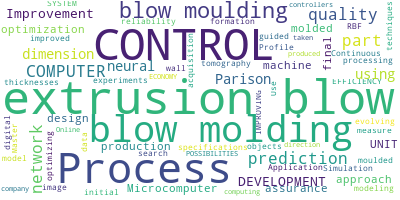
\includegraphics[scale=1]{images/chapter_2/wordcloud.png}}
\caption{Most recurrent words in article titles}
\label{fig:wordcloud}
\end{figure}

The bibliographical research work has highlighted two main strategies to improve the quality of the blow-molded parts:

\begin{itemize}
    \item Physics-based approaches: The first approach makes use of physics and simulation to model the manufacturing process and to fine tune process parameters given the simulated final part characteristics. 
    \item Data-driven approaches: As the production process is complicated to be modelled physically, most of the work carried out previously makes use of data-driven methods to understand what process parameters affect the most the quality of the blow-molded parts. The patterns discovered within data allow a subsequent optimisation of the process parameters.
\end{itemize}


In the remaining part of the current section, we will investigate the approaches proposed in the literature and we will discuss the possibility of using this methods in our industrial context. The following two subsections will provide more details about the two identified research strategies: physics-based approaches (\ref{Physics-based approaches}) and data-driven approaches (\ref{Data-driven approaches}). 

\subsection{Physics-based approaches} \label{Physics-based approaches}

Different strategies have been used to model the whole process that is the parison extrusion, clamping, inflation and cooling. \citep{lee1996prediction} used a finite element model of thin film to simulate blow molding processes, and applied the feasible direction method to minimise the parison volume at the constraints of part thickness. The proposed parison design simulation is composed of the following stages. The finite element model predicts the wall thickness of the blow-molded part from a given preform thickness. The resulting wall thickness distribution of the part is submitted to the optimisation model to generate a new preform thickness profile. The new preform design is compared with the old one. If there is any improvement, the new preform design is again passed to the finite element model, and the loop is repeated until no further design improvement can be achieved. Author showed that the presented approach makes the optimisation algorithm more efficient and reduces the computational requirement drastically. 

Others physics-based methods rely on iterative fine-tuning loop involving the prediction of the final part characteristics, such as the weight or the thickness. Two approaches, with regard to material behaviour during inflation, have been applied for the prediction. The first method assumes that the polymer melt behaves as a viscous or a viscoelastic fluid, whereas the second method assumes that the melt behaves as an elastic solid. The assumption that the parison behaves as a viscous or a viscoelastic fluid results in a very complex computational formulation. \citep{poslinski1990nonisothermal} treat the parison as a Newtonian fluid subject to a non-isothermal inflation. Parison position and cooling during the inflation are predicted as a function of time. Some experimental final part thickness distributions are obtained and compared to simulation results for a simple mould geometry and a constant initial thickness preform. Also, the inherent elastic nature of the polymer
melt is not considered, since the formulation assumes a Newtonian fluid. \cite{ryan1982dynamics} as well as \citep{khayat1992inflation} assume a viseoelastic behaviour of the polymer melt. The inflation is modelled as a dynamic process, predicting the parison inflation as a function of time. A free inflation was considered. Attempts with confined inflation, that is employing a mould geometry, have not been handled to date. 
The approaches discussed in \citep{poslinski1990nonisothermal}, \cite{ryan1982dynamics} \citep{khayat1992inflation} are interesting but make very strong assumptions or deal with very particular cases.

In 2008 \citep{attar2008manufacturing} proposed an approach to assist the development phase of a new product and to optimise the weight of the part and its thickness distribution. Firstly, simulation of the extrusion blow moulding process and preliminary experimental trials were performed concurrently to assist in the development of the part. Once the numerical modelling of the part was done, improvement of the production process was performed based upon the desired objective function, i.e., a uniform part thickness distribution and/or minimal part weight. The optimisation was performed in two sequential steps, weight optimisation then thickness optimisation, by the systematic manipulation of the operating conditions, such as the parison dimensions. A process modelling methodology was employed to demonstrate the reduction in the part development time using the new model-based approach (Figure \ref{fig:workflow_development_process_optimisation}).
\begin{figure}
\centerline{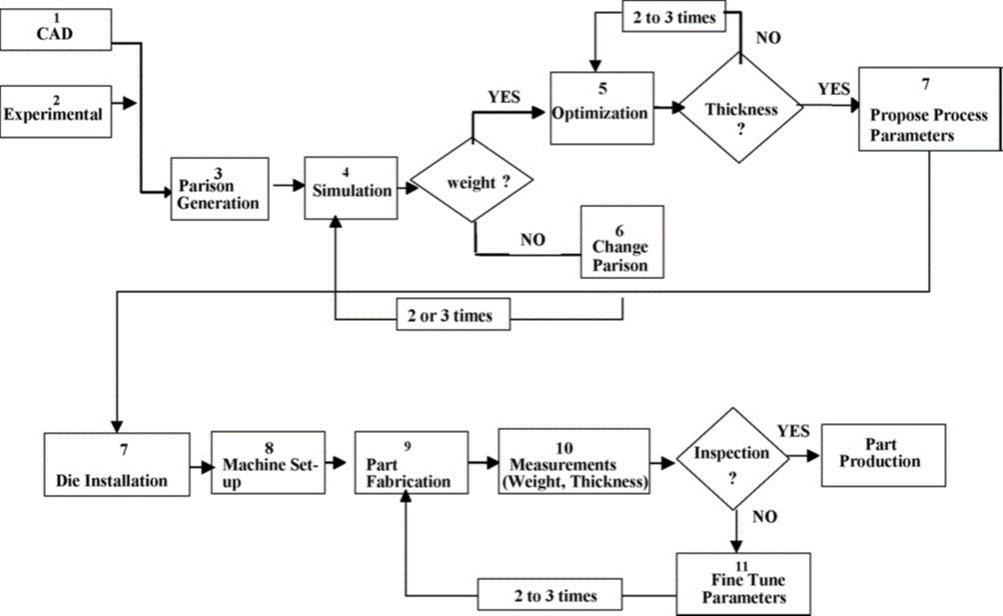
\includegraphics[scale=0.6]{images/chapter_2/optimisation_flow.png}}
\caption{Workflow for development process optimisation \citep{attar2008manufacturing}}
\label{fig:workflow_development_process_optimisation}
\end{figure}
It is a trial and error process, which is time-consuming and produces a lot of material scrap. On the other hand, the concurrent process optimises parameters virtually, and therefore, eliminates scrap, machine downtime and the need for experimental optimisation. The results demonstrate that there is a significant reduction in span time and in effort, since much of the delay and rework is eliminated using the simulation-based development process.


\subsection{Data-driven approaches} \label{Data-driven approaches}

\citep{diraddo1993line} have employed an entirely different methodology as a forward predictor of the inflation process. Neural networks are used for the on-line prediction of the final part thickness distribution from the initial process conditions. The Fully connected neural network inputs include the initial parison thickness and temperature profiles, the bottle mold geometry and a rheological parameter representative of the raw material. The neural network is trained by employing a gradient descent optimisation regression approach and mapping a broad range of output and input data. Once trained, the algorithm is capable of predicting outputs based on new inputs. Authors claimed that the proposed data-driven methods has several advantages over simulations based methods. On first principles include faster response and the network’s ability to update a model to account for process shifts. Neural networks do not allow for an understanding of process fundamentals, they require a great deal of experimental data for the training procedure and problems can arise with extrapolation beyond the range defined by the experimental
data. Therefore, the methodology is better suited for on-line applications, where fast response and following of process shifts is crucial. The same authors proposed in \citep{diraddo1993modeling} another have employed neural networks for the modelling of the process with the inverse formulation. Compared to the previous approach they tried to predict the initial parison thickness given the thickness of the final part. It would be valuable to determine the process conditions given the specified final part thickness distribution. The proposed approach was, in most cases, able to predict the constant thickness parison profile required for the specified part thickness distribution.   

Another interesting approach have been carried out by \citep{ramana2013data}. They propose to use data mining techniques to identify the factors that significantly affect quality, modeling relationships between input attributes and target attribute (yield, quality, performance index etc) and predicting quality levels of given input attributes. Clustering analysis have been initially applied on process data to split the entire population in different clusters. The cluster analysis made it possible to categorise the data into different families. By comparing the results of the cluster families analysis with the data labels, they prove that reject part are categorised in different clusters than parts conforming to customer specifications. Naive Bayes and Decision Tree has been then applied with the main purpose of classify the quality of the part given the input parameters. The process parameters used as input data are: the process cycle time, the extruder temperatures in different zones, the Extrusion Die temperature, the expulsion time, the parison length, the parison shape the blowing pressures as well as the inflation time. Naïve Bayes and clustering models were found to have better accuracy than Decision Trees in the evaluation performed by standard lift chart while predicting process parameter values that result in acceptable products. The knowledge driven and proactive decisions have been implemented in quickly setting process parameters and their range of values that resulted in increased output of high quality products and significantly reduced the scrap.

\subsection{Discussion} \label{Discussion}

The scientific literature pointed out previous works in the domain of Extrusion-Blow Molding process and quality optimisation. Two different approaches have been presented: physics-based and data-driven approaches. Both have advantages and disadvantages. Physics-based approaches need strong assumptions or simplification to account for the overall process complexity. Data-driven methods are faster and they can be used online. On the other hand, they require a great deal of experimental data for the training procedure and problems can arise with extrapolation beyond the range defined by the experimental data. Both methods try to predict the quality of the final part given the process conditions with the main purpose of fine-tuning the manufacturing process. 

This bibliographical research work has made it possible to highlight two other fundamental aspects:

\begin{itemize}
    \item Due to the complexity of the studied production process, most recent approaches to improve the quality of the manufactured parts or to improve the process control make use of data-driven methods.
    \item None of the articles considered deals with the process of multi-layers Extrusion Blow-Molding (Co-extrusion). Extrusion-Blow molding scientific literature mainly focus on plastic bottle or simple plastic containers which are commonly produced through mono-layer extrusion blow-molding process. For this reason, some of the proposed methods are not directly applicable to our production process. For instance, the approach presented by \citep{diraddo1993line} for evaluating the geometrical dimensions of a plastic bottle is really interesting. On the other hand, among the input process data used as predictors, they use the material throughput exiting the extrusion head as well as the rheological parameter representative of the raw material. This information is missing from the production process under consideration and any modification to the machine to retrieve the missing information would not be possible for technical and economical reasons.
    \item Previous research work deals mainly with the development phases of the products. Only a few of the literature works are concerned with improving the quality of the part in production. When the machine is properly set, the scrap rate is close to $0$. On the other hand, there are certain internal or external factors which can cause the production of non-conforming parts. It would be interesting to identify in real-time, or even prevent, these factors that can lead to a degradation of the product quality. This would allow a faster process adjustment and even greater reduction of the scrap rate.
\end{itemize}

 
Starting with the results obtained by \citep{diraddo1993line} and \citep{ramana2013data}, and with the advancement of machine Learning techniques in the last decade, we decided to move our attention towards data-driven methods. Supported by the scientific literature, and taking into account technological advances in the domain of the data acquisition in the manufacturing environment, we claim that data-driven methods are the right tools to investigate the interactions between Extrusion Blow-Molding process data and the corresponding product quality data. We claim that this is particularly true in a Co-extrusion production process, where there are six extrusion screws, extruding 6 different types of polymers with different physical-chemical properties. Physically modelling the production process would be quite complicated as too many assumptions would have to be taken into account. The interest of using data-driven methods is also confirmed by the scientific literature of the last years involving quality improvement. Data-driven methods for product quality control have been successfully applied in multiple domains, from steel industry \citep{lieber2013quality,li2018ensemble} to plastic industry \citep{chen2008neural,nagorny2017quality,haeussler1996quality,tellaeche2013machine,sharma2017taguchi} and to the semiconductor manufacturing processes \citep{melhem2016regression,lenz2013data,jiang2020novel}.

In the next section, some basics of machine Learning are presented with the aim of providing the reader with all the necessary elements to follow chapters 3, 4 and 5.

\section{Machine learning}

Machine learning is a field of computer science that aims to give computers the ability to learn and act without being explicitly programmed.  Traditionally, computer software is developed on the basis of a series of logical conditions constantly repeating. Instead of explicitly encoding knowledge by machine instructions, machine learning leverages data analysis, which involves building and fitting models, to allow machines to 
``learn'' from experience. Machine learning consists in building algorithms to improve the ability of machines to make predictions. Researchers and manufacturers have developed, over the years, a myriad of different kinds of Machine Learning (ML) models, or algorithms serving different situations and types of problems.

In this section we will review some concepts about machine learning in order to provide the reader with the basic elements to understand the following chapters of this PhD dissertation. Initially, some of the key concepts related to the machine learning such as difference between \textit{Supervised} and \textit{Unsupervised} learning is presented. Subsequently we will describe a few methods that have been applied all along the doctoral studies. This review is in no way intended to be exhaustive but wants to provide the necessary elements for understanding the approaches presented in chapters 3 and 4. For an exhaustive review of machine learning topics we suggest the following references: \citep{bishop2006pattern,friedman2017elements}. As regards deep learning, \citep{goodfellow2016deep} provides a comprehensive review of the most applied neural network based techniques. 


\subsection{Supervised learning}

The most widely used machine learning approach is the \textit{Supervised} one. Supervised learning is the task which involves learning a function from examples of its inputs and outputs. In supervised learning we look for a model that relates the response to the predictors, with the aim of accurately predicting the response for future observations (prediction) or better understanding the relationship between the response and the predictors (inference). In general, to solve a Supervised learning problem we look for a function that minimises an error (cost function). The cost function quantifies the overall error in prediction between the predictions of each training samples and the real value (or “grand-truth”) associated. The cost function changes depending on the problem that we want to solve: Regression or Classification.

\paragraph{Regression} \label{Regression}

Regression corresponds to a training objective where training data and their corresponding outcome, a set of numerical continuous variables, are known and available for training. More generally, suppose that we observe a quantitative response $Y$ and $p$ $(X_1,X_2,\ldots,X_p)$ different predictors. We assume that there is some relationship between $Y$ and $X = (X_1,X_2,\ldots,X_p)$, which can be written in the very general form: 

\begin{equation}
  Y=f(X) + \epsilon, \textnormal{ with } f:\mathbb{R}^{p} \rightarrow \mathbb{R}^{m}
  \enspace,
\end{equation}
where $f$ is some fixed but unknown function of $X_1,X_2,\ldots,X_p$, and $\epsilon$ is a random error term, which is independent of $X$ and has mean zero. The objective is to find an estimate of the function $\hat{f}$ that better approximates as well as possible the relationship between the response and predictors. For instance, in a manufacturing context, a regression model can be designed to predict the numerical value of some dimensional characteristic of a manufactured part, given a set of input process parameters.

\paragraph{Classification} \label{Classification}

Classification corresponds to a training objective where training data and their corresponding true outcome, called label or class, are known and available during the training phase. A machine learning model performing a classification is also called a \textit{classifier}. Its role is to infer on a label (good part/non compliant part, car/air-plane/truck, etc.) to apply to a given input data vector. The possible answers (i.e. labels or classes) are determined by the dataset given to the model during the training phase. All the possible labels need to be known during training. Given a set of $c$ different classes, an input vector composed of $p$ $(X_1,X_2,\ldots,X_p)$ different predictors, and an output vector of class probabilities $Y$, defined as follow:

\begin{equation}
    Y \in [0, 1]^{c} \textnormal{ with } \sum_{i=1}^{c} Y_{i} = 1
    \enspace,
\end{equation}
we look for the function $\hat{f}$ so that:

\begin{equation}
  Y=\hat{f}(X)+ \epsilon, \textnormal{ with } f:\mathbb{R}^{p} \rightarrow [0,1]^{c}
  \enspace,
\end{equation}

A compressed form is frequently found when there exist only two classes. This is also called \textit{binary classification}. In a manufacturing context, a classifier can be trained to recognise whether a part is compliant (OK), or not (NOK), to some quality specification.   

\paragraph{Time series classification/regression}

In some cases, we deal with several observations of the same variable over time. We define \textit{univariate time series} $T = [t_{1}, t_{2}, \dots, t_{K}]$ is an ordered set of real values. The length of $T$ is equal to the number of real values $K$. In the same way, we define an \textit{M}-dimensional Time Series, $T = [T_{1}, T_{2}, \dots, T_{M}]$ as a set of $M$ univariate time series with $T^{i} \in \mathbb{R}^{K}$. Given a dataset $D = \{(T_{1}, Y_{1}),(T_{2}, Y_{2}),\dots,(T_{N}, Y_{N})\}$ which corresponds to a collection of pairs $(T_{i}, Y_{i})$ where $T_i$ could either be a univariate or multivariate time series with $Y_{i}$ as its corresponding one-hot label vector. For a dataset containing $c$ classes, the one-hot label vector $Y_{i}$ is a vector of length $c$ where each element $j \in [1, c]$ is equal to $1$ is the class of $T_{i}$  is $j$ and \textit{0} otherwise. The task of \textit{Time series classification} consists of training a classifier on a dataset $D$ in order to map from the space of possible inputs to a probability distribution over the class variables values (labels) \citep{fawaz2019deep}. If we deal with a generic target variable $Y_{i}$, corresponding to a continous variable, the problem would take the name of \textit{Time series regression}. 


\subsubsection{Parametric models} \label{Parametric models}

Parametric models involve a two-step approach:
\begin{itemize}
    \item We make an assumption about the functional form of the function $f$.  
    \item Once the functional form is established, we need a procedure to estimate the model coefficients. 

\end{itemize}
	 
Among all parametric methods Linear Regression is the most common. The general linear function can be expressed with the following notation:

\begin{equation} \label{eq:linear_function}
    f(x)=\beta_0 + \beta_1X_1 + \beta_2X_2 + \ldots + \beta_pX_p
    \enspace,
\end{equation}
where $\beta_j$ is the generic $j$-th coefficient, associated with the $j$-th feature.
In Linear Regression, to estimate the model coefficients, we look for the hyper-plane that minimises the residual sum of squares:

\begin{equation}
    RSS = \sum_{i=1}^{n}(y_i -f(x_i))^2 = (Y - X\beta)^T(Y - X\beta)
    \enspace.
\end{equation}

Under the assumption that $X$ have full column rank, we can differentiate the equation with respect of $\beta$ to obtain the unique solution:

\begin{equation}
    \beta = (X^TX)^{-1}X^TY
    \enspace.
\end{equation}

One way to reduce the model variance is to apply a technique that constraints or regularises the coefficient estimates towards zero. The two best known methods are Ridge Regression \citep{hoerl1970ridge} and Lasso Regression \citep{tibshirani1996regression}. 

In Ridge Regression a penalty term is added to the loss function, this penalty term is also called $L2$ regularisation. The penalised residual sum of squares can be written as follows:

\begin{equation}
\begin{aligned}
 RSS_{Ridge}(\lambda) & = \sum_{i=1}^{n}(y_i -f(x_i))^2 + \lambda\sum_{j=1}^{p}\beta^{2}_{j} \\
& = \|Y - X\beta\|_2^2 + \lambda\|\beta\|_2^2
    \enspace,
\end{aligned}
\end{equation}
where $ \lambda \geq 0 $ is a complexity parameter that controls the amount of shrinkage towards zero and $||\beta||_2$ is the $L2$-norm (Euclidean norm). These parameters have to be determined separately, for example using cross-validation. The Ridge Regression coefficient estimation is given by:

\begin{equation}
    \beta_{Ridge} = (X^TX + \lambda I)^{-1}X^TY
    \enspace.
\end{equation}

Lasso Regression applies a similar shrinkage approach. In Lasso regression a penalty term ($L1$ regularisation), corresponding to an absolute value of magnitude, is applied to the residual sum of squares:

\begin{equation}
\begin{aligned}
 RSS_{Lasso}(\lambda) & = \sum_{i=1}^{n}(y_i -f(x_i))^2 + \lambda\sum_{j=1}^{p}|\beta_{j}| \\
& = \|Y - X\beta\|_2^2 + \lambda||\beta||_1
    \enspace,
\end{aligned}
\end{equation}
where $\lambda \geq 0 $ is a complexity parameter that can be estimated using cross-validation and $||\beta||_1$ is the $L1$-norm (Manhattan norm). As with Ridge Regression, the Lasso shrinks the coefficient estimates towards zero. However, the lasso penalty has the effect of forcing some of the coefficient estimates to be exactly equal to zero when $\lambda$ is sufficiently large. Lasso yields sparse models that are generally much easier to interpret than those produced by Ridge Regression. With Lasso, the features that are not related to the dependent variable are decreased towards zero so that this method is quite useful to do feature selection. Unlike Ridge Regression, however there is no closed form expression to solve the minimisation of the residual sum of squares. There are multiple algorithms for computing the entire path of solutions but their presentation is outside the scope of this paper. 

Linear, Lasso and Ridge Regression are parametric models suitable for solving Regression problems. When dealing with Classification, it is more suitable to use others approach. The most common parametric model to solve binary classification problems is \textit{Logistic Regression}. Logistic Regression is a transformation of a linear regression using the \textit{sigmoid} function: $sigmoid(x) = \frac{1}{1 + e^{-x}}$. The step from linear regression to logistic regression is kind of straightforward. In the linear regression model, we have modelled the relationship between outcome and features with a linear equation (\ref{eq:linear_function}). For classification, we prefer probabilities between $0$ and $1$, so we wrap the right side of the equation into the logistic function:

\begin{equation}
    P(Y=1) = \frac{1}{1 + e^{- (\beta_0 + \beta_1X_1 + \beta_2X_2 + \ldots + \beta_pX_p)} }
    \enspace.
\end{equation}
This forces the output to assume only values between 0 and 1.

\subsubsection{Tree-based methods} \label{Tree-based methods}

Tree based methods are simple and useful models for interpretation. These models use decision trees to determine which target value matches the observation. Decision trees split the feature space into multiple regions $R_j$ and than fit a simple model in each one. For every observation that falls into the region $R_j$ the prediction is simply the mean of the response values for the training observations in $R_j$. Another time, we look for the regions $R_j$ that minimise the residual sum of squares. Unfortunately, it is computationally infeasible to consider every possible partition of the feature space into j regions. In order to overcome this issue, we use a greedy top-down approach. The most widely used method is the CART algorithm \citep{breiman2017classification}. A CART Tree is a binary decision tree that is constructed by splitting a node into two child nodes repeatedly, beginning with the root node that contains the whole learning samples. The main idea is to grow the tree by choosing a split, among all possible splits, that maximise a defined splitting criterion. Usually the splitting criterion for regression trees is the mean squared error:

\begin{equation}
    MSE = \frac{1}{n}\sum_{i=1}^{n}(y_i -f(x_i))^2
    \enspace.
\end{equation}

Even though these model are quite good for interpretability, they are not competitive with others machine learning techniques in term of prediction. One possible way to improve the prediction capabilities is to use methods like Bagging \citep{breiman1996bagging}, Random Forest \citep{breiman2001random} and Gradient Boosting \citep{friedman2001greedy}.
With \textit{Bagging} (Boostrap Aggragation), several subsets of data are created from the training set and each of this subset is used to build a decision tree. By averaging the predictions of all the different decision trees we end up with more robust results and with the reduction of the variance of the estimated model. Given B different bootstrapped training set, the final prediction can be written as follow:

\begin{equation}
    f_{bagging}(x) = \frac{1}{B}\sum_{b=1}^Bf_b(x)
    \enspace,
\end{equation}
where $f_b(x)$ is the prediction on the $b$-th bootstrapped training set for a point $x$.
Random Forest can be seen as an extension of bagging. In addition to taking the random subset of samples, it takes a random subset of features. Once again, by averaging the results of the “Forest” generated by this method, we can obtain a more robust result compared to a single regression tree. 
Gradient Boosting is named after two different techniques: Gradient Descent and Boosting. In gradient boosting, the learning procedure consecutively fits new models to provide a more accurate estimate of the response variable. The principle idea behind this algorithm is to construct the new base-learners to be maximally correlated with the negative gradient of the loss function, associated with the whole ensemble. The loss functions applied can be arbitrary, but to give a better intuition, if the error function is the classic squared-error loss, the learning procedure would result in consecutive error-fitting \citep{natekin2013gradient}. 

\subsubsection{Support Vector Machines} \label{Support Vector Machines}

In 1992 Vapnik and coworkers \citep{boser1992training} proposed a supervised algorithm for classification that has since evolved into what are now known as \textit{Support Vector Machines} (SVMs): a class of algorithms for classification, regression and other applications that represent the current state of the art in the field.
The SVM methodology was originally conceived for binary classification problems. In a given feature space, SVM learning aims to construct a hyper-plane to best separate training data with different class labels. The hyper-plane is derived on the basis of a limited number of training instances, so-called support vectors, to maximise a margin on each side of the plane. When the samples are not linearly separable, it is possible to perform a $\Phi$ transformation, also called \textit{kernel trick} of the original data space, in order to find a space where the samples are linearly separable. The most commonly used non-linear kernels are polynomial and \textit{Radial Basis Function} (RBF) kernels.

\textit{Support vector regression} (SVR) \citep{drucker1997support}, an extension of the SVM algorithm, has been introduced for predicting numerical continuous values instead of classes. In SVR, instead of generating a hyper plane for class label prediction, a different function is derived on the basis of training data to predict numerical values. In analogy to SVM, SVR also projects training data with nonlinear structure–activity relationships in a given feature space into higher-dimensional space representations where a linear regression function may be derived.

\subsection{Unsupervised learning}

In numerous situations, collecting data and the corresponding expected output for training is too expensive or just very difficult to formalise or collect. When the objective is to design a model capable to group similar data points (i.e. clustering) without any clear predefined groups, the common approach is to explore \textit{Unsupervised Learning} (UL) methods and algorithms.

\paragraph{Clustering}

Clustering is an Unsupervised learning technique (i.e. a learning method where training data is fed into a model without the possibility to compare the output given by the model with a corresponding theoretically correct observation). Thus there is no correct answer, error or reward function, consequently the model does not rely on the availability of the domain’s experts. It is a common technique to perform knowledge discovery inside the data. Clustering focuses on finding patterns in the data to find different groups within the input data. This can be used to cluster (i.e. group) the data which are the most similar and apply later on a specific process to each of these groups.

\paragraph{Density Estimation}

Most UL objectives apart from clustering fit in a density estimation logic. One of the possible objectives with an UL could be to learn the structure of the input data distribution. Once done, a model is able to produce a new data point coming from the learned input data distribution, and thus very similar to the training data. 

This is in particular useful to create a generative model or a model able to detect any novelty, anomaly outlier data point. In many situations, there might be an interest to detect any deviation to the usual situation (e.g. IT security, dangerous situation detection, etc.). One of the common issue of these objectives is to be able to collect a representative dataset of both situation (i.e. normal and abnormal). Usually, abnormal events occur a lot less frequently, this inevitably results in an imbalanced data repartition, often by many orders of magnitude (e.g. 99.5\% normal data and 0.5\% abnormal data).


\subsection{Principal Component Analysis} \label{Principal Component Analysis}

\textit{Principal Component Analysis} \citep{pearson1901liii}\citep{hotelling1933analysis}, usually abbreviated to \textit{PCA}, is the reference dimensional reduction method that relies on a factorisation of the matrix representing the input data. Given a generic input data $X \in \mathbb{R}^{n \times p}$ the covariance matrix $C$ ca be computed as follow:

\begin{equation} \label{eq:covariance}
    C = cov(X) = \frac{1}{n - 1} \sum_{i=i}^{n} (X_{i} - \Bar{X})(X_{i} - \Bar{X})^{T}.
\end{equation}

The covariance matrix is symmetric and so it can be diagonalised:

\begin{equation}
    C = VLV^T
\end{equation}

where $V$ is the matrix of eigenevectors and $L$ is the diagonal matrix with eigenvalues. The eigenvecteurs of the covariance matrix $C$ take the name of \textit{Principal Components} of \textit{X}. The eigenvalues $\lambda_{k}$ can than be used to order the eigenvecteurs in ascending order of the variance of the data expressed by each eigenvector. By selecting $k$ Principal Components, with $k << n$ it is possible to account for most of the original dataset variability. Principal Component can be used either as a method of reducing the size of the input data space and as a Data exploratory tool. In fact, since the first Principal Components account for the most of the variability, in the majority of the cases it is possible to visualise most of the input data variability by projecting the input sample on the first 2-3 Principal Components. 


\section{Deep learning}

Deep Learning (DL) is a sub-field of ML focusing on deep neural network based architectures. DL models have become some of the top performing methods in the state-of-the-art outperforming traditional ML techniques for numerous applications and challenges. These last years have shown how deep Learning can be applied to solve multiple tasks and problems. Great improvements have been reached in multiple domains: from web searches to image recognition and classification through Convolutional neural networks to natural language preprocessing with Recurrent neural networks and \textit{Self-Attention} networks \citep{vaswani2017attention}. The democratisation of the different models through open-source software libraries, specialised chip-set and highly scalable computing platforms has pushed companies to integrate these tools within their own production facilities. The deep learning research is advancing very fast and new architectures are proposed every day. An exhaustive overview of DL is out of the scope of this research work but, in the following subsection we will introduce three different families of neural networks: Feed-forward neural network, Convolutional neural network and Recurrent neural network, as well as some specific architectures that we will applied in chapter 4.


\subsection{Neural network}

A neural network is a computing system made up of a number of simple, highly interconnected processing elements (units). Feed-forward neural networks learn to map a fixed-size input to a fixed-size output. To go from one layer to the next, the units compute a weighted sum of their inputs from the previous layer and pass the result through a non-linear function (activation function). For a generic hidden layer $H$ of a neural network the $j$-th unit compute the following operation:  

\begin{equation}
    h_j^H = \sigma(\sum_{i \in H-1}W_{ij}x_i)
    \enspace,
\end{equation}
where $W_{ij}$ is the weight on connection from unit $j$ and the $i$-th unit of the previous layer, and $\sigma$ is the activation function. Among all activation functions the most popular on these days are \textit{ReLu} (Rectified Linear Unit) \citep{Glorot2011DeepSR}, which is defined as follow:

\begin{equation}
    ReLu(x) = max(0,x)
    \enspace.
\end{equation}

Without the activation function the neural network would be a stacking of linear models and it would not be able to take into account non-linear connections between inputs and outputs. 
Units that are not in the input or output layer are conventionally called hidden units. The hidden layers can be seen as distorting the input in a non-linear way so that categories become linearly separable by the last layer \citep{DBLP:journals/nature/LeCunBH15}. During the training phase we compute an objective function that measures the error (or distance) between the output scores and the desired pattern of scores. The back-propagation algorithm uses the derivative chain rule to calculate the gradient of an objective function with respects to the weights of a multilayer stack of units. In other words, the gradient of the objective function with respect to the inputs can be computed by working backwards from the gradient calculated with the respect of the output. The gradient, for each weight, indicates by what amount the error would increase or decrease if the weight were increased by a tiny amount. Once the gradient is propagated to the input, it is used to upgrade the unit weight through the use of optimisation algorithms. The most common optimisation algorithm is the Stochastic Gradient Descent (SGD). With SGD multiple samples of the training set are used to compute the output and the corresponding error. The error with respect to the weights is calculated and the weights are updated with following equation:

\begin{equation}
    W_j = W_j - \eta\nabla C(W_j)
    \enspace,
\end{equation}
where $\eta$ is the learning rate, the “step size” with we which we descend the gradient, and $\nabla C(W_j)$ is the gradient of the cost function with respect to the weights.
In the last few years others optimisation algorithms have been proposed. Among them the most widely used are \textit{RMSprop} and \textit{Adam} (adaptive moment estimation) \citep{kingma2014adam}

\subsection{Convolutional neural network} \label{Convolutional Neural Network}

Convolutional Neural Networks (CNN) are neural networks that use convolutions in place of general matrix multiplications in at least one of their layers. 
\begin{figure}
\centerline{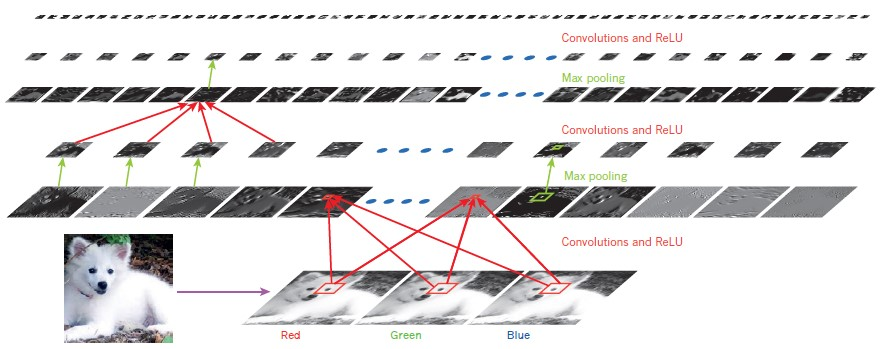
\includegraphics[scale=0.7]{images/chapter_2/CNN.jpg}}
\caption{Convolutional network overview \citep{DBLP:journals/nature/LeCunBH15}}
\label{fig:cnn_overview}
\end{figure}
The architecture of a typical ConvNet (Figure \ref{fig:cnn_overview}) is structured as a series of stages. The first few stages are composed of two types of layers: convolutional layers and pooling layers. Units in a convolutional layer are organized in feature maps, within which each unit is connected to local patches in the feature maps of the previous layer through a set of weights called a filter bank. The result of this local weighted sum is then passed through a non-linearity such as a ReLU. All units in a feature map share the same filter bank. Different feature maps in a layer use different filter banks.

CNN have three great properties which are well suited for processing data that has a known grid-like topology: “sparse interactions”, “parameter sharing” and “equivariant representations” \citep{goodfellow2016deep}. Compared to traditional fully connected layers where every output unit interacts with every input unit, CNNs have sparse interactions. In fact, the size of the convolutional kernel is lower than the size of the input data which means that we need to store fewer parameters, which both reduces the memory requirements of the model and improves its statistical efficiency. Moreover, the same kernel is used throughout grid-like input data, so instead of learning a parameter for each location, only a set of parameters is
learnt. This drastically reduce the number of parameters to learn. With the "equivariant representations" we means the property of CNNs to be equivariant to translations. This implies that if we translate an object in an input image, also its representation produced through the convolutional operation would be translated of the same amount. This property is particularly interesting when we know that some function of a small number of neighboring pixels is useful when applied to multiple input locations. The properties presented above make CNN particularly suitable for working with images. 

Among the many possible applications involving CNNs we remember \textit{Image Classification}, \textit{Object Detection}, \textit{Instance segmentation} and \textit{Semantics segmentation}. Image Classification is a fundamental task that attempts to comprehend an entire image as a whole. The aim is to classify the image by providing it a label. Image Classification often refers to images in which just one item appears and is analysed. Object detection, on the other hand, involves both classification and localisation tasks and is used to analyse more realistic scenarios in which numerous items may exist in an image. Advanced computer vision tasks, instance segmentation, are intended to achieve finer-grained object localisation in input images. The bounding boxes used in object detection find only coarse-grained object boundaries and include many pixels that do not belong to the object. In contrast, instance segmentation improves the object localisation accuracy by identifying each pixel that acts as part of a known object in the image. The semantic segmentation task involves associating each pixel in an image with a class label. In the following subsections we will review 3 different Convolutional based architecture we have used in the course of our research work: \textit{Residual networks} (image classification), \textit{Single Shot MultiBox Detector} (object detection) and \textit{U-Net} (image segmentation).

\subsubsection{Residual networks} \label{Residual Networks}

Most of the state-of-the-art Image classification methods use Residual networks, better known as \textit{ResNet}\citep{he2016deep}. The ResNet architecture solves the vanishing gradient problem for very deep neural network architectures by applying the concept of residual learning. By applying \textit{Shortcut connections} (Figure \ref{fig:shortcut}) it is possible for gradients to propagate further and allow for efficient training of very deep neural networks.

\begin{figure}
\centerline{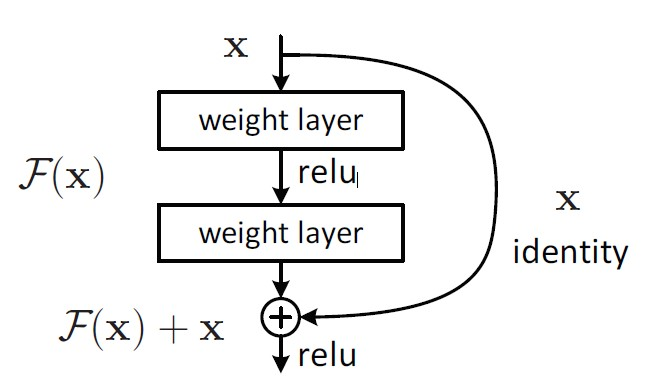
\includegraphics[scale=0.5]{images/chapter_2/residual_learning.jpg}}
\caption{Shortcut \citep{he2016deep}}
\label{fig:shortcut}
\end{figure}

There is empirical evidence that Residual networks are easier to optimise, and can gain accuracy from considerably increased depth. By stacking multiple convolutional layers and by leveraging the concept of residual learning, Residual networks may be very depth with more than 100 convolutional layers. Depending on the number of Convolutional layers, there exists multiples versions of the these models. The most popular architectures are \textit{ResNet18}, \textit{ResNet34}, \textit{ResNet50}, \textit{ResNet101}, \textit{ResNet152}. As shown in figure \ref{fig:resnet_architectures}, the generic ResNet\textit{X} is composed of 5 convolutional building blocks and a last fully connected layer which leverage the extracted features to produce the classification result. Depending on the depth of the architecture each convolutional building is composed of a different number of convolutional layers.

\begin{figure}
\centerline{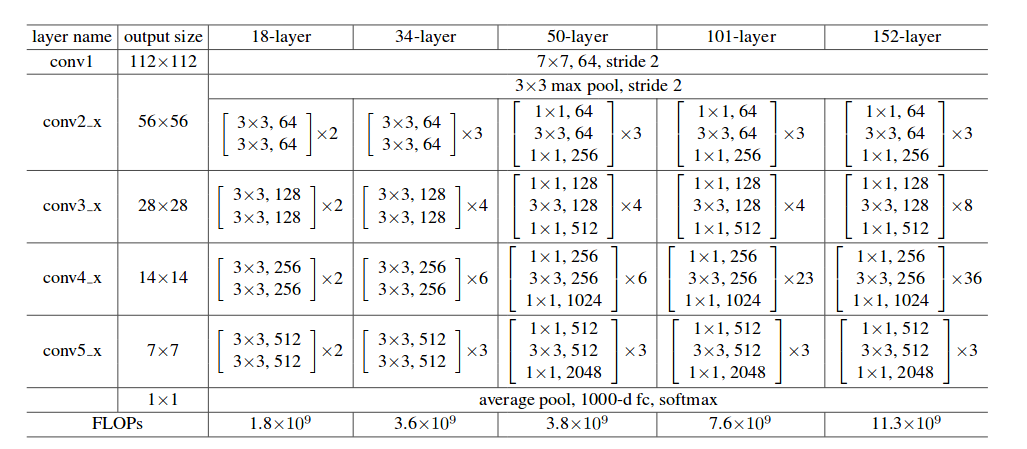
\includegraphics[scale=0.4]{images/chapter_2/resnet.png}}
\caption{ResNet architectures \citep{he2016deep}}
\label{fig:resnet_architectures}
\end{figure}


\subsubsection{Single Shot MultiBox Detector}

Single Shot MultiBox Detector (SSD) (Figure \ref{fig:ssd_architecture}) is a single-stage object detection method that discretizes the output space of bounding boxes into a set of default boxes over different aspect ratios and scales per feature map location \citep{liu2016ssd}. At prediction time, the network generates scores for the presence of each object category in each default box and produces adjustments to the box to better match the object shape. Additionally, the network combines predictions from multiple feature maps with different resolutions to naturally handle objects of various sizes.

\begin{figure}
\centerline{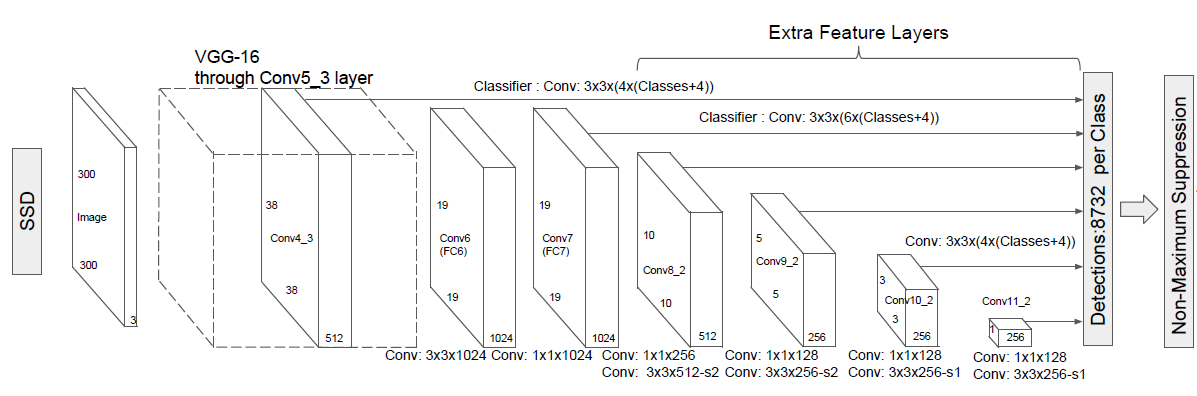
\includegraphics[scale=0.45]{images/chapter_2/ssd_network.png}}
\caption{SSD Architecture \citep{liu2016ssd}}
\label{fig:ssd_architecture}
\end{figure}

This model mainly consists of a base network followed by several multi-scale feature map blocks. The base network is for extracting features from the input image, so it can use a deep CNN. For example, the original single-shot multibox detection paper adopts a \textit{VGG network} \citep{simonyan2014very} truncated before the classification layer. In recent years, other base network architectures have been combined with the multi-scale feature maps blocks. \textit{MobileNet} has been developed to speed up the computation and lends itself well to being combined with the SSD model to perform Object Detection tasks in real-time.  

MobileNet networks \citep{howard2017mobilenets, sandler2018mobilenetv2, howard2019searching} are a family of general purpose computer vision neural networks designed with mobile devices in mind to support classification, detection and more. The popularity these architecture is motivated by the the overall trade-off between the inference speed the model performances.
The main idea behind MobileNet models is based on the concept of \textit{depth-wise separable convolutions}. Depth-wise separable convolutions is a form of factorised convolutions which factorise a standard convolution into a depth-wise convolution and a $1\times1$ convolution called a point-wise convolution. For MobileNets the depth-wise convolution applies a single filter to each input channel. The point-wise convolution then applies a $1\times1$ convolution to combine the outputs the depth-wise convolution. A standard convolution both filters and combines inputs into a new set of outputs in one step. The depth-wise separable convolution splits this into two layers, a separate layer for filtering and a separate layer for combining. This factorisation has the effect of drastically reducing computation and model size \citep{howard2017mobilenets}.


\subsubsection{U-Net}

One popular approach for semantic segmentation models is to follow an encoder/decoder structure where we “downsample” the spatial resolution of the input, developing lower-resolution feature mappings which are learned to be highly efficient at discriminating between classes, and the “upsample” the feature representations into a full-resolution segmentation map. The encoder-decoder approach, as part of the semantic segmentation domain, was proposed for the first time by \citet{long2015fully} in the Fully Convolutional Network (FCN) architecture and it has been subsequently taken up by other research works \citep{ronneberger2015u,zhao2017pyramid,chen2017rethinking,chen2018encoder,badrinarayanan2017segnet}. The encoder, or contracting path, is, most of the time, a Convolutional neural network whose task is to extract features of different spatial resolutions, constituting the so-called “Feature Map”. Compared to the encoder, which reduces the spatial dimension in every layers and increases the channels, the decoder, or expansive path, has the role of restoring the original spatial dimensions by sequentially increasing the spatial dimension while reducing the number of channels. The decoder can be composed of one of multiple decoder block, in the same way the encoder can be more or less deep. Each decoder block computes two different operations: at first it up-sample the feature map using an interpolation method, then it applies a convolutional operation which halves the number of feature channels. Finally, a last convolutional block, sometimes called Segmentation Head, stacked right after the last decoder block produces the segmentation mask. 

One architecture that follows this approach is the \textit{U-net} architecture (Figure \ref{fig:unet_architecture}, proposed by \citep{ronneberger2015u}.
\begin{figure}
\centerline{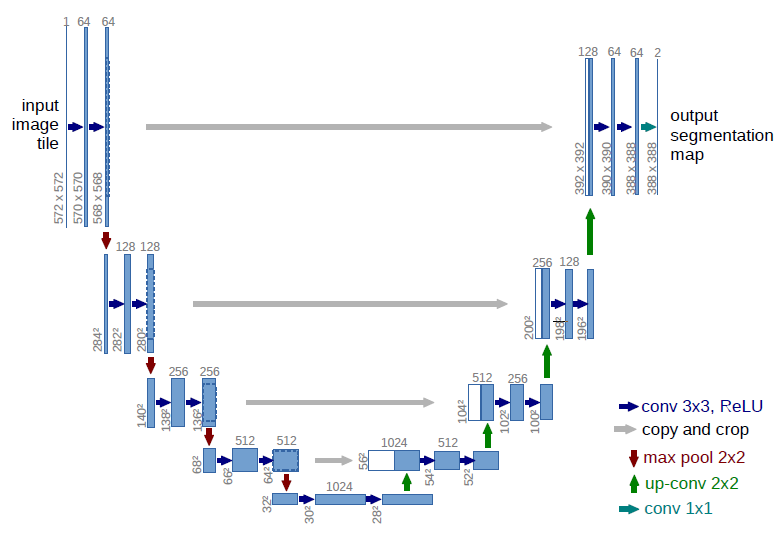
\includegraphics[scale=0.6]{images/chapter_2/unet.png}}
\caption{U-net architecture \citep{ronneberger2015u}}
\label{fig:unet_architecture}
\end{figure}
It consists of a contracting path (left side) and an expansive path (right side). The contracting path follows the typical architecture of a convolutional network. It consists of the repeated application of two 3x3 convolutions (unpadded convolutions), each followed by a rectified linear unit (ReLU) and a 2x2 max pooling operation with stride 2 for downsampling. At each downsampling step we double the number of feature channels. Every step in the expansive path consists of an upsampling of the feature map followed by a 2x2 convolution (“up-convolution”) that halves the number of feature channels, a concatenation with the correspondingly cropped feature map from the contracting path, and two 3x3 convolutions, each followed by a ReLU. The cropping is necessary due to the loss of border pixels in every convolution. At the final layer a 1x1 convolution is used to map each 64-component feature vector to the desired number of classes. In total the network has 23 convolutional layers.

Even if this architecture has been surpassed by more complex methods, constitutes a good trade-off between results accuracy and model complexity, allowing its use in contexts where the size of the training set is not particularly large.


\subsection{Recurrent neural networks} \label{Recurrent Neural Network}

Recurrent Neural Networks (RNN) \citep{rumelhart1986learning} are a family of neural networks that possess internal state or short-term memory due to recurrent feed-back connections, that make them suitable for dealing with sequential problems. The main advantage of RNN compared to others neural network architectures is their ability to process sequences of any length by keeping into account the historical information. More effective sequence models used in practical applications are called \textit{gated RNNs}. These include the \textit{LSTM} (Long-Short-Term-Memory) \citep{hochreiter1997long} and \textit{GRU} (gated recurrent unit) \citep{cho2014properties}. Without going into much details, gated RNNs are based on the idea of creating paths through time that have derivatives that neither vanish nor explode \citep{goodfellow2016deep}. The LSTM has been found extremely successful in many applications, such as speech recognition \citep{graves2013hybrid}\citep{graves2014towards}, machine translation \citep{sutskever2014sequence} and image captioning \citep{kiros2014unifying}\citep{vinyals2015show}\citep{xu2015show}. Thanks to its ability to deal with sequential data, RNN based networks have also been applied reasonably to time series regression/classification tasks \citep{smirnov2018time}.  

\section{Model Hyper-parameters fine-tuning}

The algorithms presented in the previous section have several dozen hyper-parameters. Their adjustment is often crucial to obtain a satisfactory performance. This is called hyper-parameter optimisation: the aim is to optimise the performance of the model for the task at hand. It is also necessary to select the right data preparation methods. This is particularly true for deep learning architectures when the number of hyper-parameter is important. Table \ref{tab:hyper-parameters} summarises the most critical Hyper-parameters to fine tune while training a deep neural network.

\begin{table}[]
\label{tab:hyper-parameters}
\begin{tabular}{|l|p{4cm}|p{4cm}|}
\hline
\textbf{Hyper-parameter}           &  \textbf{Common values applied in scientific literature}  & \textbf{Description}                                    \\ \hline
Number of layers          & {[}2;200{]}                                     & Number of layers in the architecture.           \\ \hline
Layer type                & Fully-connected, Convolutional, Recurrrent, ... & Neural network layer family                                               \\ \hline
Number of Neuron per layer & {[}1;4000{]}                                    & Number of Neuron composing a layer.                                               \\ \hline
Activation function       & ReLu, Softmax, Sigmoid, Tanh, ...               & Function which define the output of the neuron in a range of values.                                                \\ \hline
Cost function             & MSE, MAE, \textit{Hinge} Loss, Categorical cross-entropy, \dots                                                & Function which measure the error between the prediction and the ground truth value.                                               \\ \hline
Weight initialisation     & Random initialisation, \textit{Xavier} initialisation \cite{glorot2010understanding}, \textit{He} initialisation \citep{he2015delving}, \dots                                                & The method applied to initialize model weights. \\ \hline
Learning rate             & {[}$10^{-10}$;$10^{-1}${]}                                                  &  Amount that the weights are updated during training.                                               \\ \hline
Mini-batch                & {[}2;256{]}                                     & Equally sized subset of data over which the gradient is calculated and weights updated.                                               \\ \hline
\end{tabular}
\caption{Most known Hyper-parameters for training a deep neural network}
\end{table}

Methods for automatic optimisation of these hyper-parameters have been proposed. There exists today many Open Source optimisation frameworks that allows to perform this optimisation tasks in an easy manner. Among them we can mention \textit{Optuna} \citep{optuna_2019} that we have used throughout our research work. \textit{Optuna} provides an easy interface to automate the hyper-parameter search. It supports the following sampling algorithms: \textit{Grid and Random Search} (\ref{Grid and Random search}), \textit{Tree-structured Parzen Estimator} (\ref{TPE approach}).


\subsection{Grid and Random search} \label{Grid and Random search}

In order to perform the optimisation, the performance of the method over the range of values of each of the hyper-parameters needs to be evaluated. It is possible to evaluate the whole value range exhaustively, by a regular test grid, which is computationally expensive. A less costly approach in term of calculation time is the random drawing over the range of values, proposed by \citep{bergstra2012random}. 
\begin{figure}
\centerline{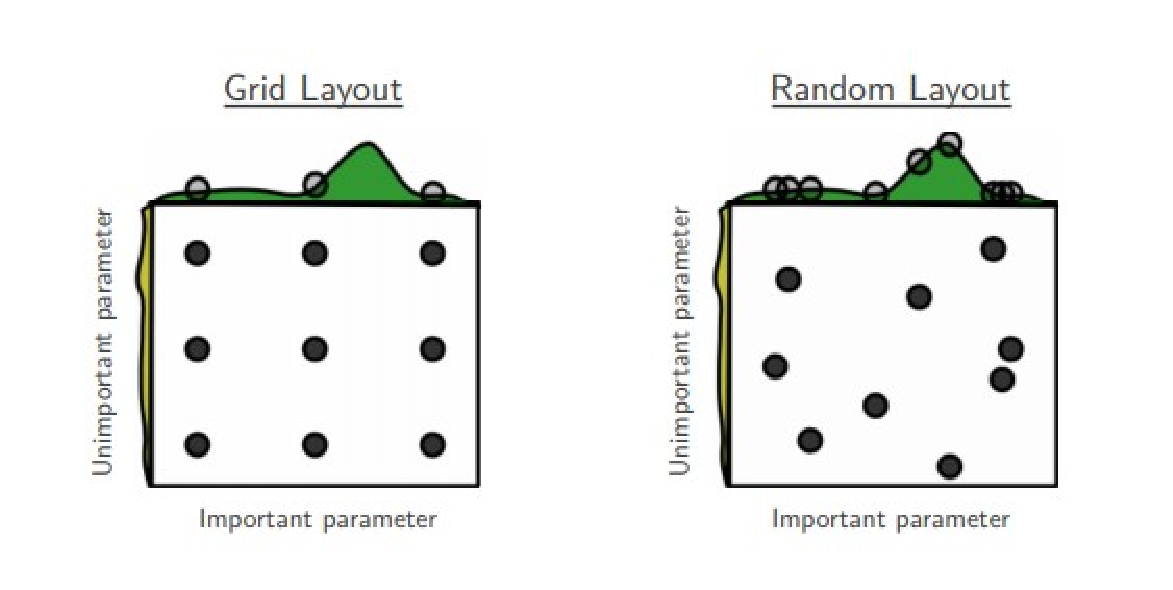
\includegraphics[scale=0.7]{images/chapter_2/random_search.eps}}
\caption{Grid and Random Search \citep{bergstra2012random}}
\label{fig:Grid and Random Search}
\end{figure}
In Figure \ref{fig:Grid and Random Search} the Grid search and Random search of nine trials are compared for optimising a generic function $f(x, y) = g(x) + h(x)$ where Above each square $g(x)$ is shown in green, and left of each square $h(y)$ is shown in yellow. With grid search, nine trials only test $g(x)$ in three distinct places. With random search, all nine trials explore distinct values of $g$. This failure of grid search is the rule rather than the exception in high dimensional hyper-parameter optimisation.

\subsection{Iterative Methods}

In 2011, \citep{bergstra2011algorithms} carried out a state of the art of hyper-parameter optimisation methods for deep neural network models. This work shows the interest of iterative optimisation, based on the criterion of the Expected Improvement of the model performance, proposed by \citep{jones2001taxonomy}. The study introduces two optimisation methods. One method seeks to model the optimisation problem by \textit{Gaussian stochastic processes} (GP) and the second TPE (\textit{Tree-structured Parzen Estimator}) method proposes a kernel-based modeling. These methods are based on the construction of meta-models. The study highlighted the superiority of these two methods over the optimisation by random sampling. In the context of this research work we applied solely the TPE algorithm.

\paragraph{TPE approach} \label{TPE approach}

The Tree-structured Parzen Estimator (TPE) is a sequential model-based optimisation (\textit{SMBO}) approach. SMBO methods sequentially construct models to approximate the performance of hyper-parameters based on historical measurements, and then subsequently choose new hyper-parameters to test based on this model. The TPE approach models $P(x|y)$ and $P(y)$ where x represents hyper-parameters and y the associated quality score. $P(x|y)$ is modelled by transforming the generative process of hyper-parameters, replacing the distributions of the configuration prior with non-parametric densities.

In this subsection we have shown how the hyper-parameters can be optimised. Whether it is carried out through a Random sampling approach or through the use of iterative methods, hyper-parameter optimisation it is an expensive task in term of computation time. The cost of optimising these models is very high, due to the infinity of possible architectures and the many hyper-parameters, especially for neural networks. In the following subsection, we will present an approach that allows for reducing the overall computational time and which facilitates the convergence of the model, especially if the number of samples composing the training set is not particularly high.


\subsection{Transfer Learning} \label{Transfer Learning}

Transfer learning is biologically motivated by the way that humans apply learned knowledge to solve new problems, and consists in exploiting knowledge learned in one problem and searching a good protocol of transferring to a new problem.
In practice, in transfer learning problems, a parametric model is trained in the source problem and transferred to the target problem in a special way, like transferring parameters, or considering the relations between problems. This approach become particularly interesting when we deal with a dataset where the number of samples is small. There is no a well-defined rule to distinguish between a small and a large dataset. Moreover, the amount of data required to solve a machine Learning problem depends on the task that we try to accomplish. In the context of this research project we consider as small, every dataset that have less than 1000 samples. 

Convolutional networks are broadly applicable in the fields mentioned before. The success of transfer learning with convolutional networks relies on the generality of the learned representations that have been constructed from a large database like ImageNet \citep{deng2009imagenet}. \citep{yosinski2014transferable} quantified the transferability of these pieces of information in different layers, e.g. the first layers learn general features, the middle layers learn high-level semantic features and the last layers learn the features that are very specific to a particular task. \citep{zeiler2014visualizing} also visualised the features in the intermediate layers, demonstrating, with images, that convolutional networks learn features from general level to task-specific level. Overall, the learned representations can be conveyed to related but different domains and the parameters in the network are reusable for different tasks. The intuition behind transfer learning for image-related tasks is that if a model is trained on a large and general enough dataset, this model will effectively serve as a generic model of the visual world. You can then take advantage of these learned feature maps without having to start from scratch by training a large model on a large dataset.

In practice, we distinguish two successive stages in the training of a neural network by transfer learning: the training of the new last layers, and then the specialisation of the whole network. The first stage is to guarantee the convergence of the classifier on the new task. We seek to obtain a satisfactory inference score. This is why in a first step, only the weights of the neurons of the new last layers are adjusted by back-propagation of the error gradient. Once the convergence of the last layers has been obtained, it is possible to fine-tune the whole network by performing an adjustment of all the weights of the layers in order to improve the classification score.


\section{Conclusion TO BE FINISHED}

% This chapter allowed us to present our first contributions. A review of the literature on process control and quality improvement in the context of Extrusion Blow-Molding.

\subsection{Scientific Contribution TO BE FINISHED}

\subsection{Industrial Contribution TO BE FINISHED}


